\documentclass{sigchi}

% Use this command to override the default ACM copyright statement (e.g. for preprints). 
% Consult the conference website for the camera-ready copyright statement.


%% EXAMPLE BEGIN -- HOW TO OVERRIDE THE DEFAULT COPYRIGHT STRIP -- (July 22, 2013 - Paul Baumann)
% \toappear{Permission to make digital or hard copies of all or part of this work for personal or classroom use is         granted without fee provided that copies are not made or distributed for profit or commercial advantage and that copies bear this notice and the full citation on the first page. Copyrights for components of this work owned by others than ACM must be honored. Abstracting with credit is permitted. To copy otherwise, or republish, to post on servers or to redistribute to lists, requires prior specific permission and/or a fee. Request permissions from permissions@acm.org. \\
% {\emph{CHI'14}}, April 26--May 1, 2014, Toronto, Canada. \\
% Copyright \copyright~2014 ACM ISBN/14/04...\$15.00. \\
% DOI string from ACM form confirmation}
%% EXAMPLE END -- HOW TO OVERRIDE THE DEFAULT COPYRIGHT STRIP -- (July 22, 2013 - Paul Baumann)

% Arabic page numbers for submission. 
% Remove this line to eliminate page numbers for the camera ready copy
% \pagenumbering{arabic}


% Load basic packages
\usepackage{balance}  % to better equalize the last page
\usepackage{graphics} % for EPS, load graphicx instead
\usepackage{times}    % comment if you want LaTeX's default font
\usepackage{url}      % llt: nicely formatted URLs
\usepackage{subcaption}

% llt: Define a global style for URLs, rather that the default one
\makeatletter
\def\url@leostyle{%
  \@ifundefined{selectfont}{\def\UrlFont{\sf}}{\def\UrlFont{\small\bf\ttfamily}}}
\makeatother
\urlstyle{leo}


% To make various LaTeX processors do the right thing with page size.
\def\pprw{8.5in}
\def\pprh{11in}
\special{papersize=\pprw,\pprh}
\setlength{\paperwidth}{\pprw}
\setlength{\paperheight}{\pprh}
\setlength{\pdfpagewidth}{\pprw}
\setlength{\pdfpageheight}{\pprh}

% Make sure hyperref comes last of your loaded packages, 
% to give it a fighting chance of not being over-written, 
% since its job is to redefine many LaTeX commands.
\usepackage[pdftex]{hyperref}
\hypersetup{
pdftitle={SIGCHI Conference Proceedings Format},
pdfauthor={LaTeX},
pdfkeywords={SIGCHI, proceedings, archival format},
bookmarksnumbered,
pdfstartview={FitH},
colorlinks,
citecolor=black,
filecolor=black,
linkcolor=black,
urlcolor=black,
breaklinks=true,
}

% create a shortcut to typeset table headings
\newcommand\tabhead[1]{\small\textbf{#1}}


% End of preamble. Here it comes the document.
\begin{document}

\title{Mining Attendee Data to Improve Academic Conferences}

\numberofauthors{3}
\author{
  \alignauthor 1st Author Name\\
    \affaddr{Affiliation}\\
    \affaddr{Address}\\
    \email{e-mail address}\\
    \affaddr{Optional phone number}
  \alignauthor 2nd Author Name\\
    \affaddr{Affiliation}\\
    \affaddr{Address}\\
    \email{e-mail address}\\
    \affaddr{Optional phone number}    
  \alignauthor 3rd Author Name\\
    \affaddr{Affiliation}\\
    \affaddr{Address}\\
    \email{e-mail address}\\
    \affaddr{Optional phone number}
}

\maketitle

\begin{abstract}
One of the primary goals of academic conferences is to promote scientific exchange of advances among people who may otherwise not have the opportunity to hear from one another. Conference organizers put time and effort in various activities such as putting papers in thematically coherent sessions, ensuring related papers are not scheduled at the same time, planning various events to bring together people with shared interests, choosing speakers, etc.  They often struggle to gather all the information necessary to do these right. Despite all the efforts from conference organizers it is still not easy for attendees to find and attend all the papers/talks they want to see, and meet/exchange ideas with other attendees who share similar interests as theirs.

We present \emph{Confer}, a tool designed to help conference attendees find interesting papers/talks, discover/meet people with shared interests, and manage their time using a personalized schedule for the conference. So far, we have deployed Confer to 13 academic conferences including CHI, CSCW, KDD, ACM MM, SIGMOD, SIGIR, and WSDM. Our log analysis and survey results show that the tool helps conference attendees find interesting papers, manage schedule, and discover other attendees with shared interests. We explore how the large-scale usage data of the tool can help plan various conference organization activities such as scheduling sessions, forming communities and sub-communities, assigning speakers, planning community interactions, etc., and present a case for a data-driven decision making for academic conferences.
\end{abstract}

\keywords{
        data-driven conference planning; confer.
}

\category{H.5.m.}{Information Interfaces and Presentation (e.g. HCI)}{Miscellaneous}

\section{Introduction}
A primary role of academic conferences is to bring together people with shared interests to exchange ideas and knowledge. Conference attendees go to academic conferences with two major goals -- a) see papers/talks relevant to their interests, and b) meet and exchange ideas with other people who share similar interests. Conference organizers do their best to facilitate these needs -- they try to create thematically relevant sessions (to help attendees find papers/talks relevant to their interest) and schedule them in a way that will minimize conflicts for attendees (papers an attendee wants to see shouldn't be scheduled at the same time in parallel); they plan various events/activities to bring people with shared interests together to meet and exchange ideas.  For logistic and pragmatic reasons, it typically becomes a responsibility of a few dedicated organizers ~\cite{EventPlanning}. Organizers often struggle to \emph{gather all the information necessary to do it right} and despite their best effort they often fail to accommodate unforeseen issues and unvoiced opinions~\cite{CoDesign}.

We present Confer, a tool designed to help attendees find relevant papers/talks, meet people with shared interests, and manage their time efficiently using a personalized schedule for their conference. Conference attendees use Confer to search for papers (Figure~\ref{confer-search}) and explore by browsing through recommended papers (Figure~\ref{confer-similar-papers}). While exploring, they add interesting papers to their preference list (Figure~\ref{confer-recommendations}). Confer automatically creates a personalized schedule (Figure~\ref{confer-personal-schedule}) based on their preference list which they use to manage their time at the conference. We launched the tool in April 2013 for CHI 2013, and since then have hosted 13 academic conferences including CHI, CSCW, KDD, ACM MM, SIGMOD, SIGIR, and WSDM. Over the last 18 months, the tool has been used by more than 18,000 attendees. 6,600 attendees have registered accounts on confer. To understand how useful the tool is for attendees, we analyzed the usage data and conducted surveys. Our analysis indicates that the tool helped attendees find relevant papers/talks, meet other attendees with shared interests, and manage their time efficiently using their personalized schedule.

Confer collects natural, rich preference data on how attendees plan to spend their time at the conference. Attendees use the tool for their own benefit, but the collective data can help organizers and the community. We argue for a data-driven approach towards conference planning. We explore how we can use the natural, rich preference data gathered from the usage of the tool. We describe various experiments we ran at CHI 2014 to evaluate the feasibility of using the data. The data can be mined to gain insights into the structure of shared interests, community, sub-communities, different areas of research, new/emerging areas, etc. We show that the data is valuable for various conference planning activities such as scheduling sessions, choosing speakers, creating program committees, planning community interactions, etc.

The contributions of the paper are as follows:
\begin{itemize}
\item Confer, a web-based conference navigation interface for attendees to discover relevant papers/talks, meet other attendees with shared interests, and navigate the conference using a personalized schedule.
\item An analysis of the usage data and user surveys demonstrating the usefulness of the tool for conference attendees.
\item An argument for a data-driven conference planning with exploration of various use-cases, with the case study of CHI 2014.
\end{itemize}

This paper is organized as follows. First, we describe the system, various design decisions, and how it helps attendees find relevant papers/talks and meet other people with similar interests. Next, we discuss our analysis of usage data and attendees' responses to the surveys we conducted. We then explore the data gathered from the usage of the tool and how the data can be useful to help conference organizers make important decisions. In the end we discuss the possible implications of data-driven decision making for academic conferences.

\section{Related Work}
Confer is a tool that collects natural, rich preference data on how attendees plan to spend their time at the conference. We look at how the data collected as a by-product of a natural exploration by conference attendees can be used for making various decisions in conference planning.

Conference Navigator ~\cite{ConferenceNavigator}, Conferator ~\cite{ConferenceAnatomy}, and Confex ~\cite{Confex} are other tools designed to help conference attendees find relevant papers/talks. We try to pursue gathering attendees' preferences prior to holding (or scheduling) the conference so that the data can be used for planning the conference itself. We explore how we can use the data gathered as a by-product of natural exploration by conference attendees to various use-cases in conference planning. The use-cases we present can make use of data generated by other tools too.

Cobi~\cite{CobiUIST2013} is a tool that pursues gathering data prior to scheduling the conference. It collects data from authors by inviting the authors of the accepted papers to identify papers that would fit well in a session with their own, and which papers would they like to see. Attendee-Sourcing ~\cite{AttendeeSourcingHCOMP14} shows that the data gathered as a by-product of natural exploration by attendees are of very different nature than the data collected by Cobi from authors. The data collected from Confer and Cobi complement each other.

The idea of leveraging large-scale user interaction data organically generated from users' collective behaviors has been an active area of research in the HCI community. Read wear~\cite{Hill:1992:EWR:142750.142751} collects users' natural document browsing behaviors to augment the scrollbar with visitation frequency information, Patina~\cite{patina} collects personal and community usage data of a GUI to visualize and recommend menu items of the user's interest, and LectureScape~\cite{lecturescape} uses video watchers' video player interaction data (e.g., play, pause clicks) to support various information needs to improve the navigation experience of educational videos. Confer contributes to this line of research with using usage data in the unique domain of academic conferences. Also, previous research has focused on collecting usage data from applications, users are already familiar with (e.g., reading a page, watching educational videos, using Word for document editing), but with Confer, we create the application itself that did not exist for the target population in addition to collecting and using the data.

There is an active area of research in matchmaking. Confer contributes to this area of research by providing APIs which can be used by tools/applications targeting conference attendees. CommonTies \cite{Abouzied:2014:CCN:2556420.2556783} is a simple technological nudge that uses context-aware profile-matching system to encourage social interactions among strangers. The profile matching system of CommonTies is powered by Confer Meetups APIs.

Collaborative filtering is a method of making automatic predictions about the interests of a user by collecting preferences or taste information from many other similar users ~\cite{CollaborativeFiltering}. It has proven to be valuable for recommending items in many different domains. CitationRecommendation ~\cite{CitationRecommendation} has explored the use of collaborative filtering to recommend research papers, using the citation web between papers to create the ratings matrix. We recommend new papers/talks to attendees using the attendees' marked papers to construct the ratings matrix.


\section{System Description}
\subsection{Design Goals}
Confer is a web-based application primarily designed to help conference attendees a) discover relevant papers/talks, b) meet people who share similar interests, and c) manage their time efficiently using a personalized schedule. Responsive design is applied to support small-screens and smartphones. In this section, we describe the interface and the design rationale in detail.


\textbf{Design Goal 1. Discover Relevant Papers}\\
The goal is to make it easy for attendees to find papers they would want to see. Confer supports three main affordances for discovering relevant papers/talks.

\emph{Discovery by search:} Attendees can search using keywords (any word in the title, abstract, author, paper-keywords, etc.) to find papers matching the keywords in the query (Figure~\ref{confer-search}). This interface is important for attendees to find and mark papers they already know they want to see. From our logs we find that attendees search for papers from a particular institution/organization, papers by a particular author, papers related to a particular topic, etc. 

\begin{figure}[!h]
\centering
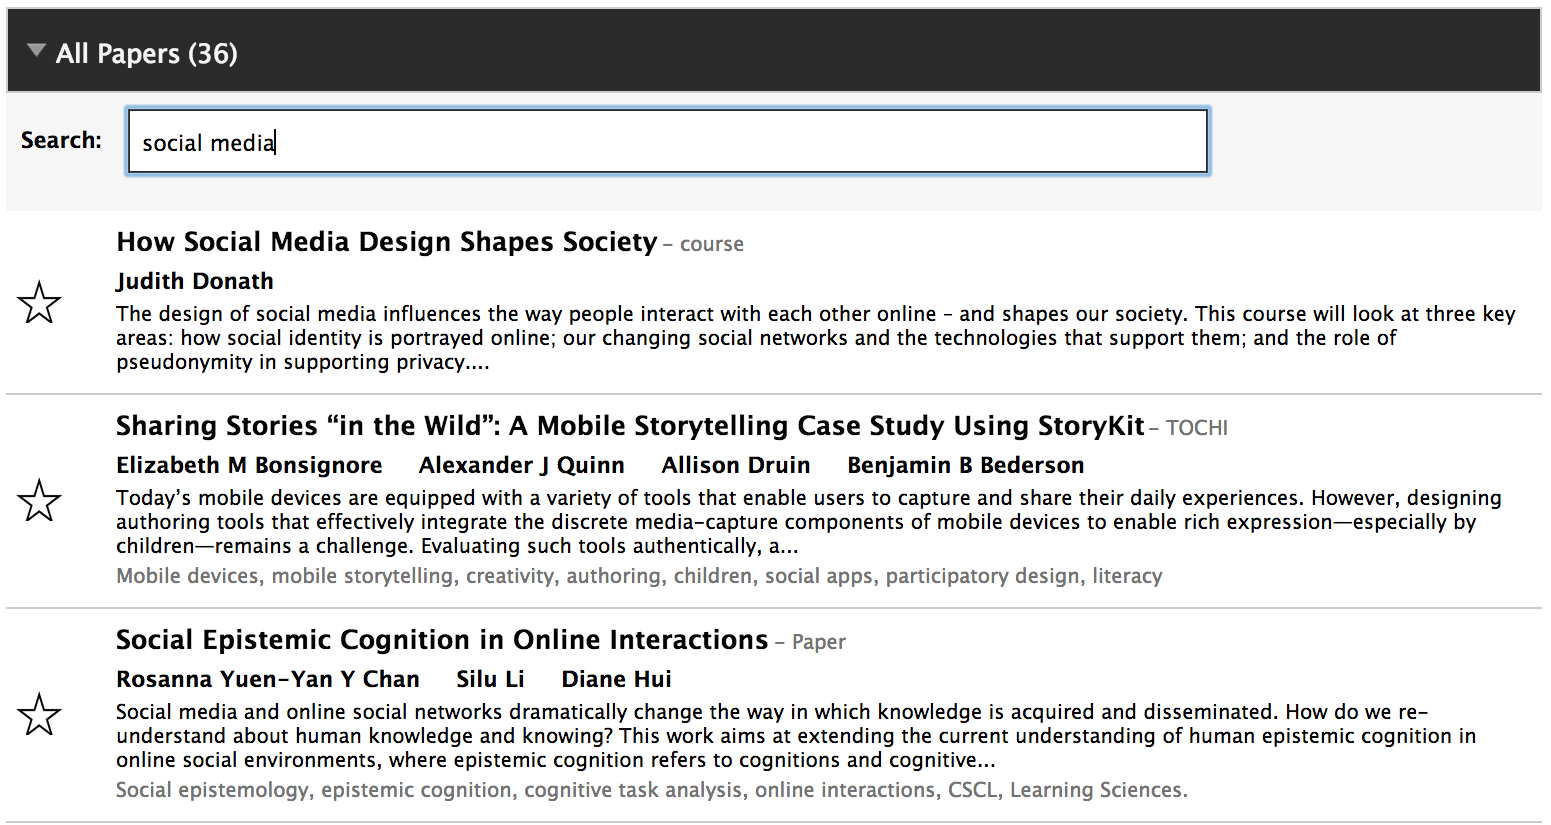
\includegraphics[width=0.95\columnwidth]{confer-search.png}
\caption{Attendees can search for papers using keywords, author names, affiliation, etc.}
\label{confer-search}
\end{figure}

\emph{Discovery while exploring:} When an attendee clicks on a paper to explore (read more about the paper), we show the paper's abstract and a list of other papers similar to the selected paper (Figure~\ref{confer-similar-papers}). Showing the list of similar papers helps attendees navigate to other papers similar to the selected paper. We consider ``opening a paper for reading'' as an implicit signal for the user's next navigation. Our log analysis suggests that a user is more likely to navigate to a paper similar to the one the user is currently looking at. This interface is designed to help attendees quickly navigate to another paper/talk related to the one they are currently looking at.
\begin{figure}[!h]
\centering
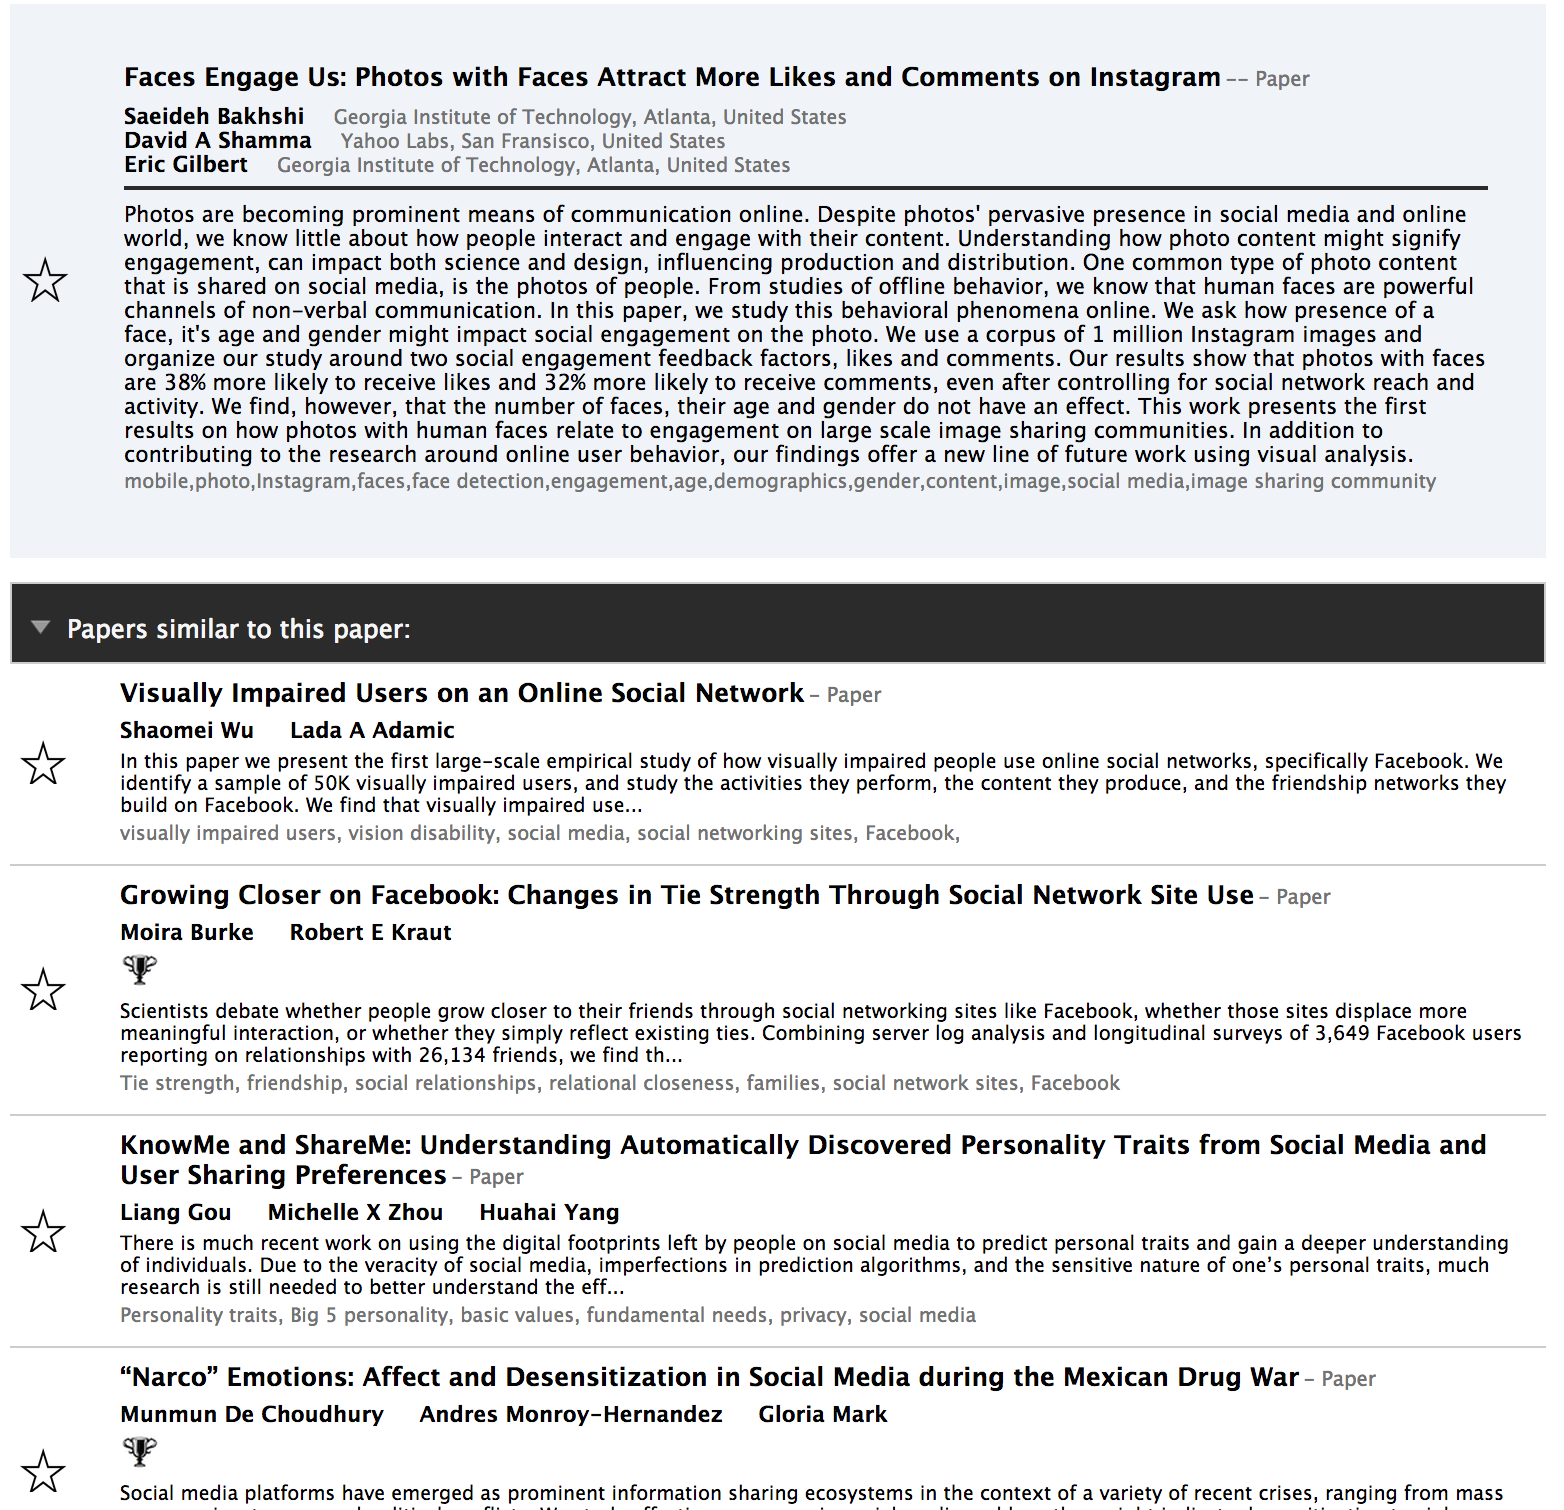
\includegraphics[width=0.95\columnwidth]{confer-similar-papers.png}
\caption{Attendees see similar papers while exploring a paper of interest.}
\label{confer-similar-papers}
\end{figure}


\emph{Discovery by looking at the recommendations:} Attendees can mark a paper as ``interested in seeing'' by starring it. This adds the marked paper to their ``interested in seeing'' list. For each attendee, we generate a personalized set of recommendations based on the papers the attendee has already marked as ``interested in seeing'' (Figure~\ref{confer-recommendations}). The recommendations are dynamic and they automatically get refreshed when either the attendee adds/removes a paper from her/his ``interested in seeing'' list, or the changes in the community network cause the recommendations to change. The social recommendations help attendees discover new papers in their interest area. The interest area for an attendee is inferred by looking at all the papers he/she has already marked as ``interested in seeing''.
\begin{figure}[!h]
\centering
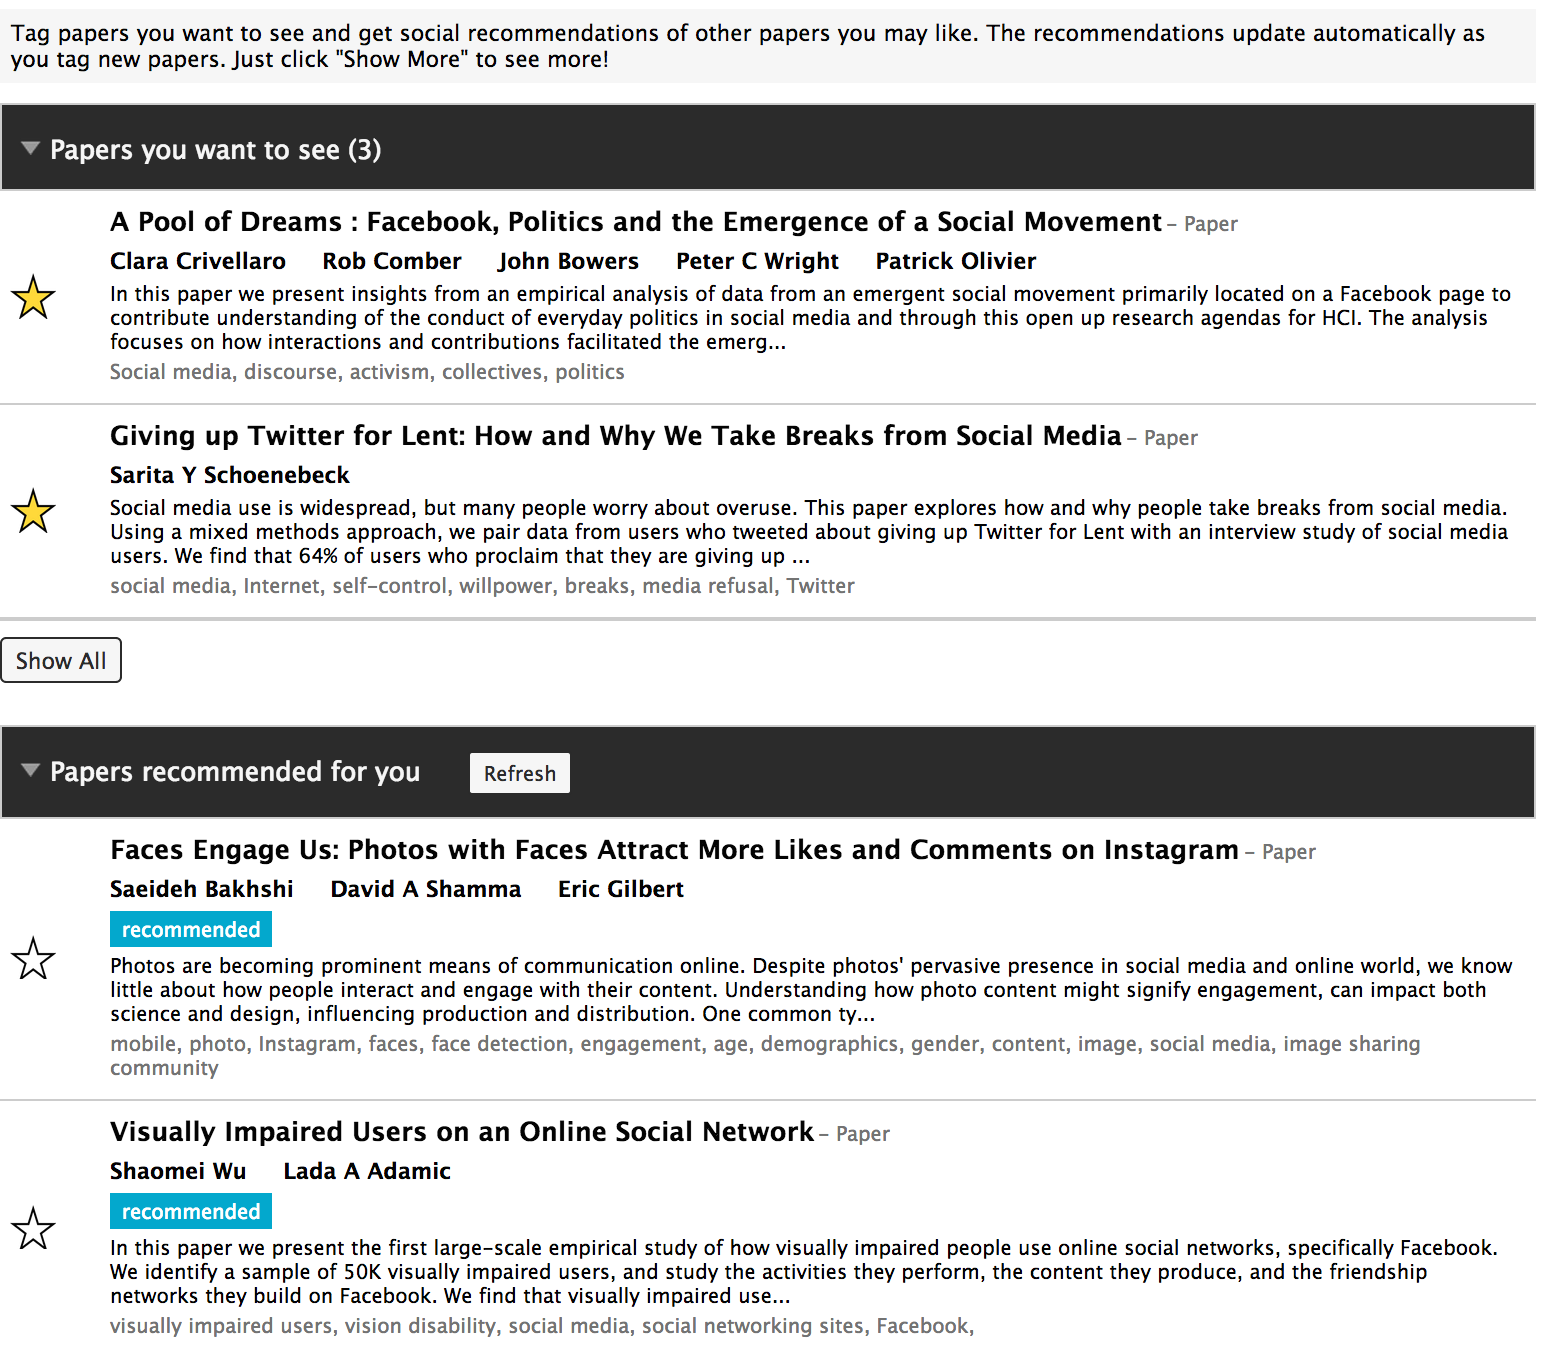
\includegraphics[width=0.95\columnwidth]{confer-recommendations.png}
\caption{Attendees are presented with a set of recommendations based on their current selection to help them discover relevant papers.}
\label{confer-recommendations}
\end{figure}

\textbf{Design Goal 2. Meeting People with Shared Interests}\\
Another important goal of Confer is to encourage attendees with shared interests to meet and exchange ideas. Since attendees mark papers they are interested in seeing, we can compute similarity between attendees by looking at their preferences. For each attendee, we can now show a list of other attendees with similar interests. There are two important design considerations though:
\begin{figure}[!h]
\centering
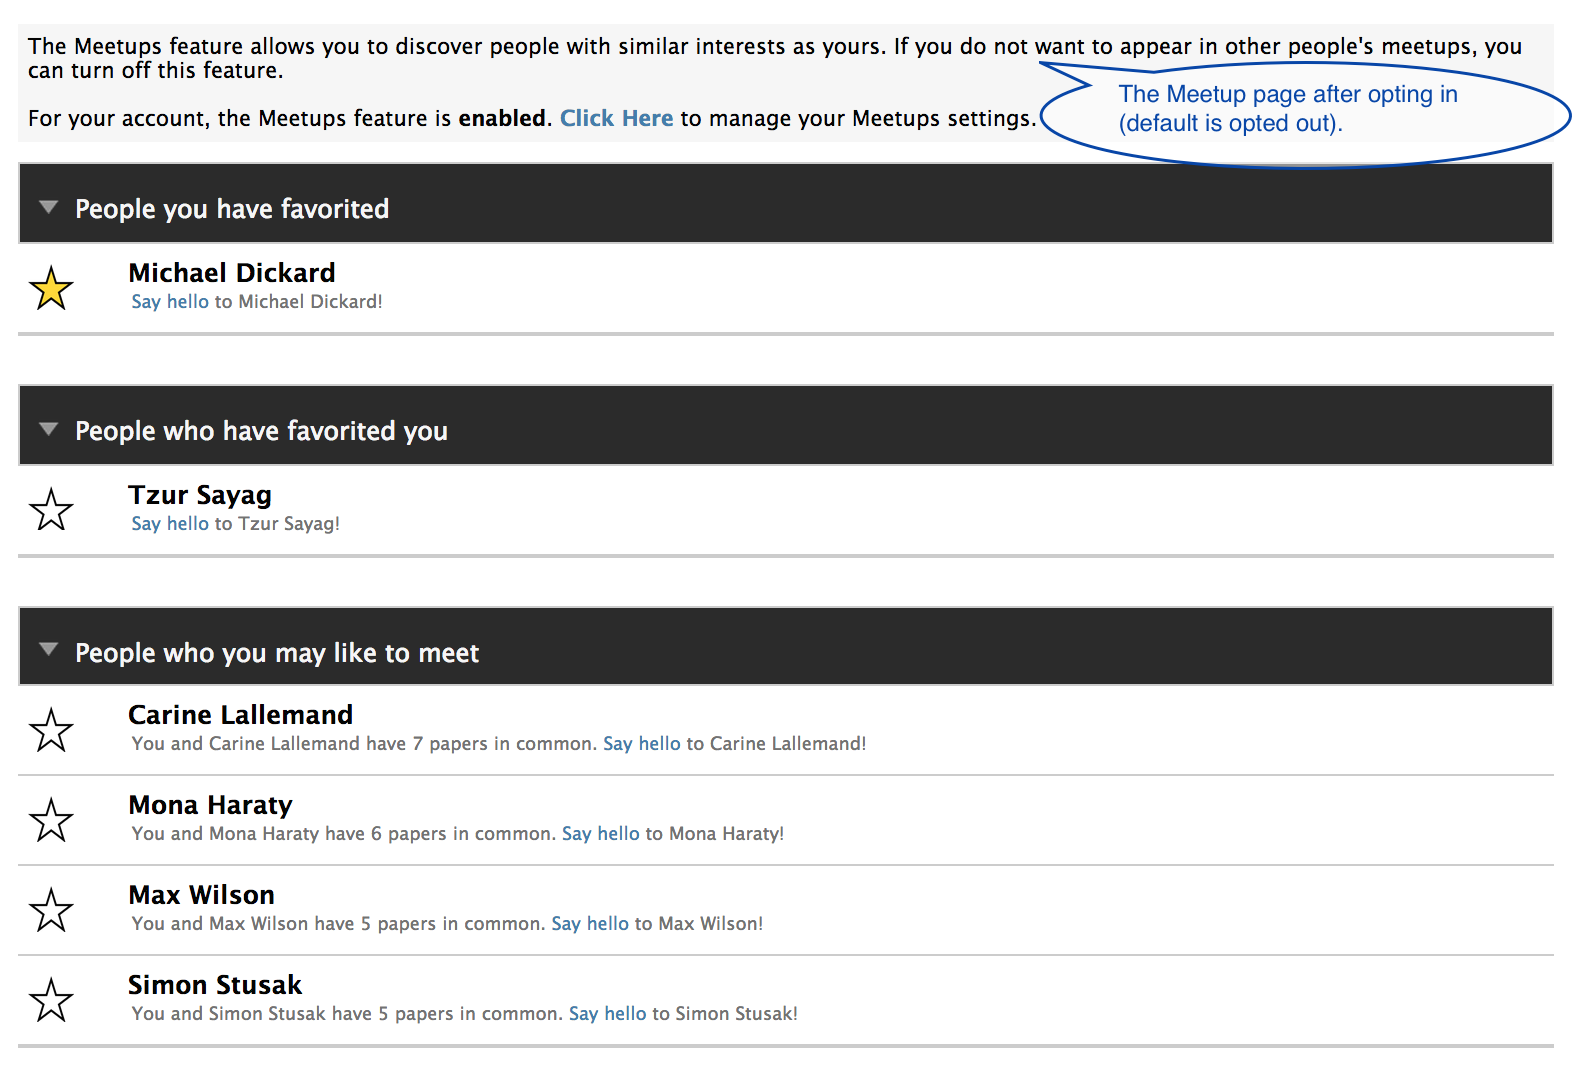
\includegraphics[width=0.95\columnwidth]{confer-meetup.png}
\caption{Confer interface to help attendees meet other people with shared interests.}
\label{confer-meetup}
\end{figure}
\begin {itemize}

\item \emph{Privacy}:  People are usually not comfortable receiving an email from a stranger asking to meet. For this reason we made a decision to keep this as an ``opt-in'' feature with a default of ``opted out'' (Figure~\ref{confer-meetup}). We do not show any attendee as a recommendation to other attendees unless the attendee has explicitly opted in the Meetups functionality. We recommend only those attendees as recommendations who have explicitly opted in.

\item \emph{Initial communication barrier}: Even after explicit opt in, we realize that there is an initial barrier in starting a communication. Attendees do not feel comfortable taking the initiative of sending an email to someone they do not know. To reduce this barrier, we put a ``Star'' icon next to each recommended person. Attendees can add a person to their ``Favorite'' list by clicking on the Star icon next to the person in the interface (Figure~\ref{confer-meetup}). Once an attendee favorites a person from the recommended list, the system sends a notification to the person favorited. If the person favorites back the attendee, then it becomes socially less awkward for the two to exchange email and meet. We did A/B test and our log analysis concludes that attendees are more likely to use the ``favoriting'' interface to initiate the communication. We discuss our log analysis in detail later in the paper.
\end {itemize}

\textbf{Design Goal 3. Personalized Scheduling for Conference Attendees}\\
To help attendees manage their time at the conference, we generate a personalized schedule for them. The personalized schedule for an attendee is generated based on all the papers the attendee has marked as ``interested in seeing'', and the papers recommended by our recommendation system. We provide a set of filters that allows attendees to see different views of their personalized schedule and make an informed decision about where they should spend their time.

\begin{figure}[!h]
\centering
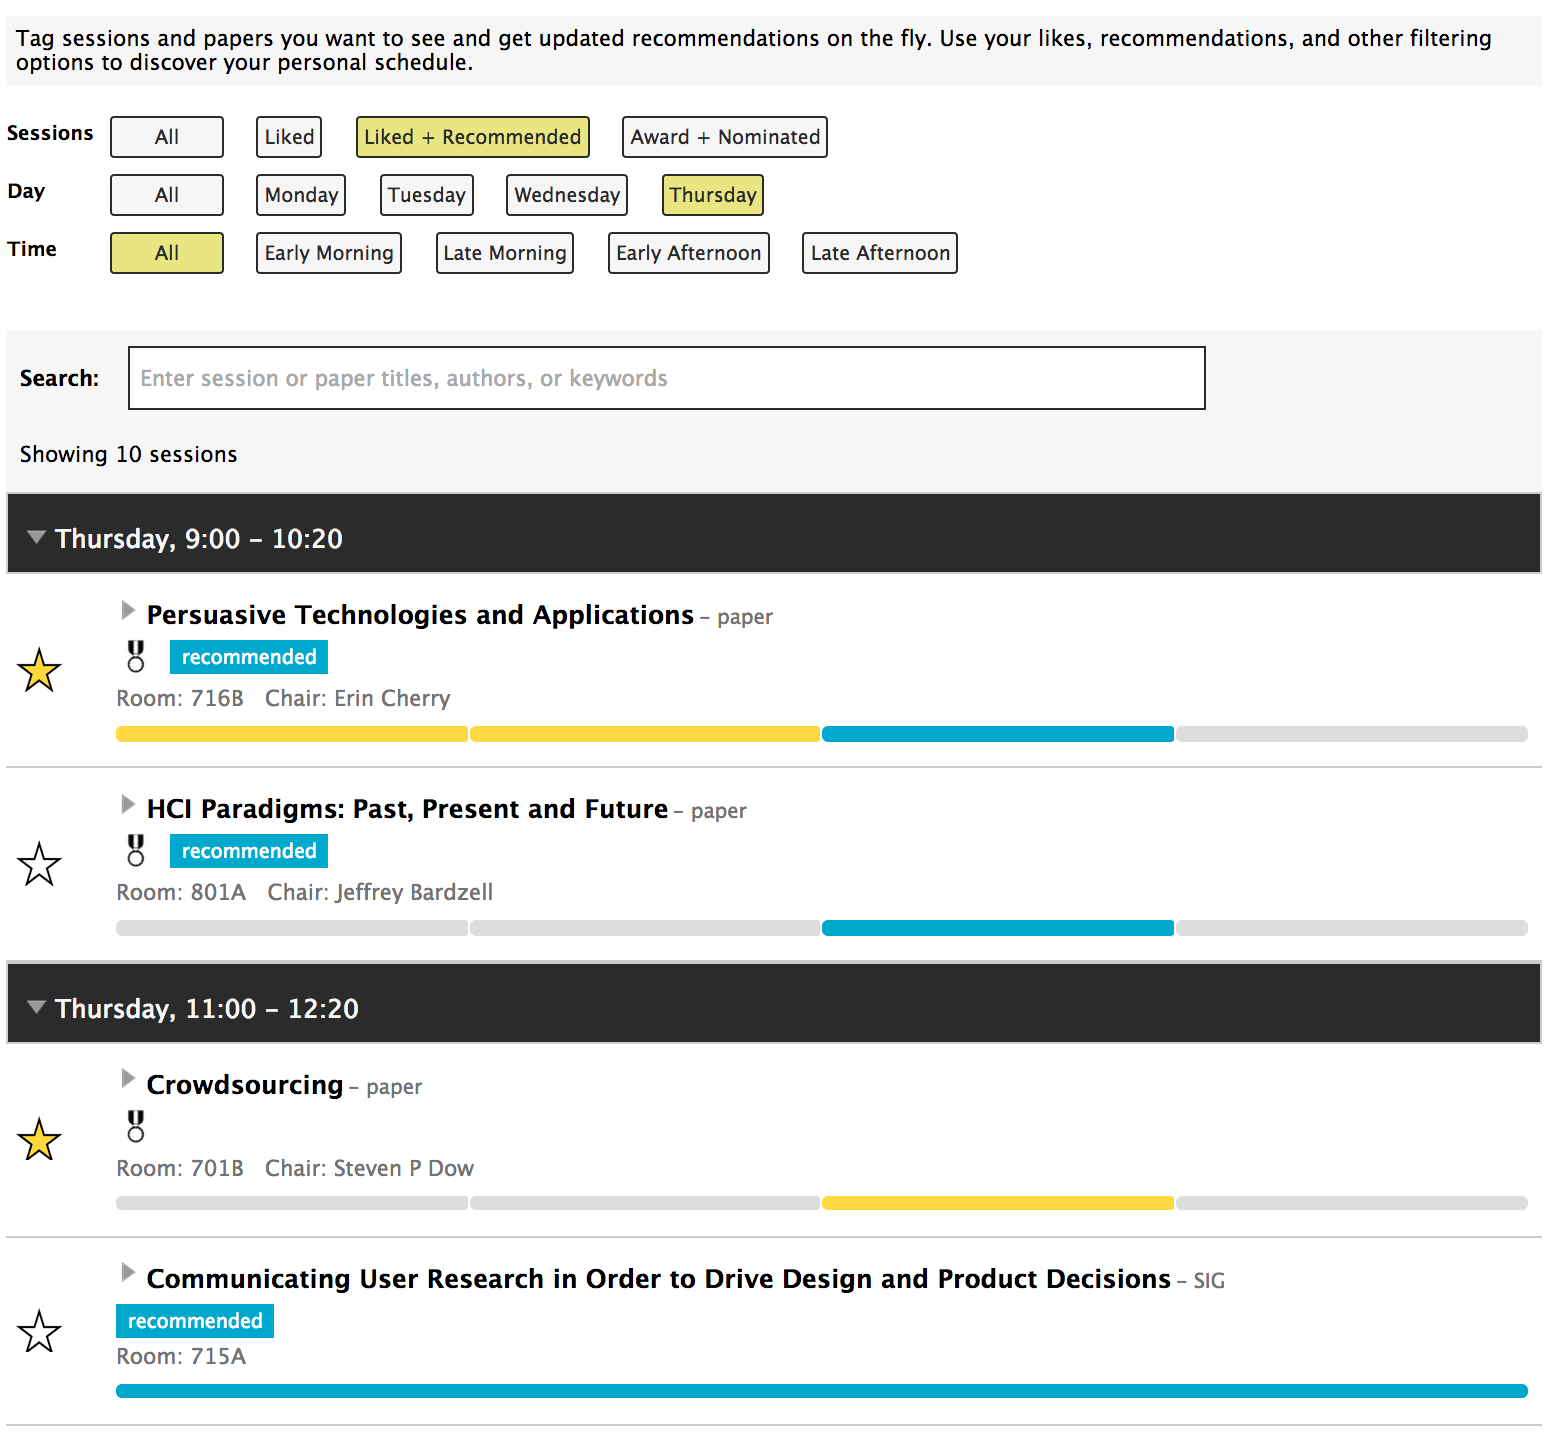
\includegraphics[width=0.95\columnwidth]{confer-personal-schedule.png}
\caption{Confer creates a personalized schedule for attendees.}
\label{confer-personal-schedule}
\end{figure}

\subsection{Implementation Details}
For recommending papers, Confer uses collaborative filtering ~\cite{CollaborativeFiltering} based social recommendations. Collaborative filtering is a method of making automatic predictions about the interests of a user by collecting preferences or taste information from many other similar users. The idea is to automatically find similar attendees in the community, and then recommend new papers/talks to attendees based on the fact that other similar attendees liked the papers/talks. In the beginning, when there aren't enough preferences to support collaborative filtering, the system automatically falls back to content-based (TF-IDF) recommendations. This bootstrapping ensures that attendees always get some relevant recommendations when they open Confer. The design goal is to keep the attendees engaged by showing them papers they are most likely to find interesting.

There are a number of different mathematical formulations that can be used for finding similar people. We use cosine-based similarity, also known as vector-based similarity. To find similarity between two attendees, we take the papers they are interested in seeing as two vectors. The similarity between the two attendees is computed as the cosine of the angle between the two vectors. 

\subsection{Deployment \& Usage}
Confer has been running since April, 2013 and so far we have hosted 13 academic conferences including CHI, CSCW, KDD, ACMMM, SIGMOD, SIGIR, and WSDM. Some of these conferences have been hosted twice.

\emph{Tool Usage:} The app has been used by more than 18,000 attendees. 6,600 attendees have registered accounts on Confer. Out of 6,600 registered accounts, 5239 have starred at least 1 paper. We consider only these 5239 users in our analysis. They marked a total of 114, 472 preferences (interested in seeing) with an average of 21.85 preferences per user (std-dev: 19.7, median: 15, min: 1, max: 155). On an average, a paper appears in the preference list of 21.94 (std-dev: 11.87, median: 21, min: 0, max: 156) attendees. The most popular paper appeared in the preference list of 156 attendees. While these numbers vary for each conference, the variation is not too much and thus we do not report the usage for each individual conference.

\emph{Usage of Paper Recommendations:} On an average, 63.8\% (median 66.45, std-dev: 14.76) of the ``papers interested in seeing'' list came from clicking on recommendations. Rest of the papers in the list were starred from the search results and the schedule page.

\emph{Meetups Usage:} The Meetups feature, recommending people with similar paper interests inside Confer, has been launched recently, and we have only activated it for three conferences - CSCW 2014, CHI 2014, and KDD 2014 so far. As of now,  a total of 436 users (21.8\% of the total registered users for these conferences) explicitly enabled the Meetups functionality. There are 139 pairs with both-way favoriting (a pair favorited papers by each other), and 179 pairs with one-way favoriting (only one side favorited the other in a pair). Because of some problem in our system, we don't have the exact numbers of emails exchanged. Also, we do not know how many of these pairs really met in person.

Confer data has also been used by other tools/applications targeting conference attendees. 
CommonTies ~\cite{Abouzied:2014:CCN:2556420.2556783}, a simple technological nudge that uses context-aware profile-matching system to encourage social interactions among strangers was deployed at CSCW 2014. The profile matching system of CommonTies was powered by Confer Meetups APIs.

\section{Survey Results \& Log Analysis}

We log all the user activities to understand how Confer users use the system. However, to complement the usage statistics with a more qualitative understanding, we conducted a web-based survey that conference attendees could voluntarily participate in. The survey responses from various conferences have been aggregated. There were a total of 247 attendees who responded to the survey. Since the Meetups feature was activated recently, we have only 103 responses for meetups-related questions (Figure~\ref{survey-responses}).

\begin{figure}[!h]
\centering

\begin{subfigure}[t]{0.9\columnwidth}
\centering
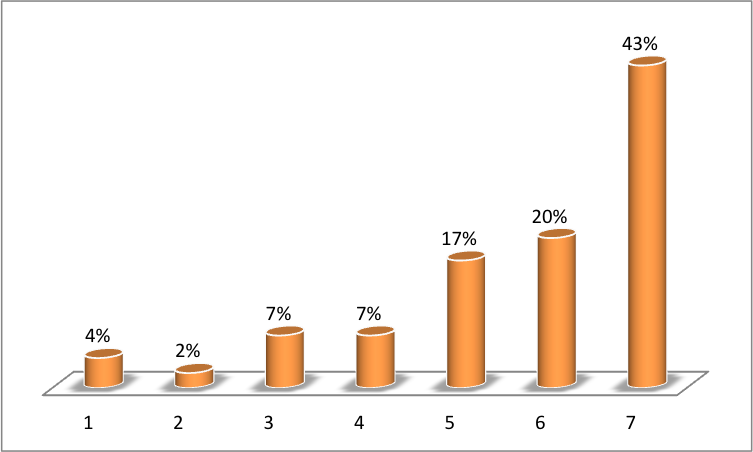
\includegraphics[width=0.9\columnwidth]{survey-q-1.png}
\caption{Distribution of 247 responses to ``did you find Confer useful?''}
\label{survey-q-1}
\end{subfigure}

\vspace{10pt}
\begin{subfigure}[t]{0.9\columnwidth}
\centering
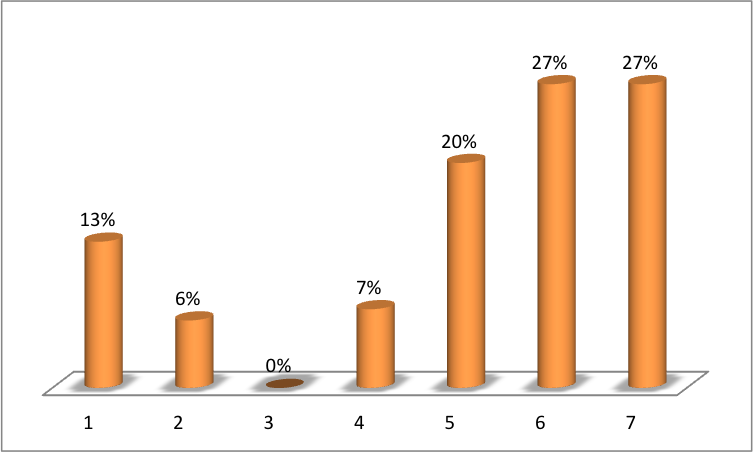
\includegraphics[width=0.9\columnwidth]{survey-q-2.png}
\caption{Distribution of 247 responses to ``were the recommendations relevant and helpful?''}
\label{survey-q-2}
\end{subfigure}

\vspace{10pt}
\begin{subfigure}[t]{.9\columnwidth}
\centering
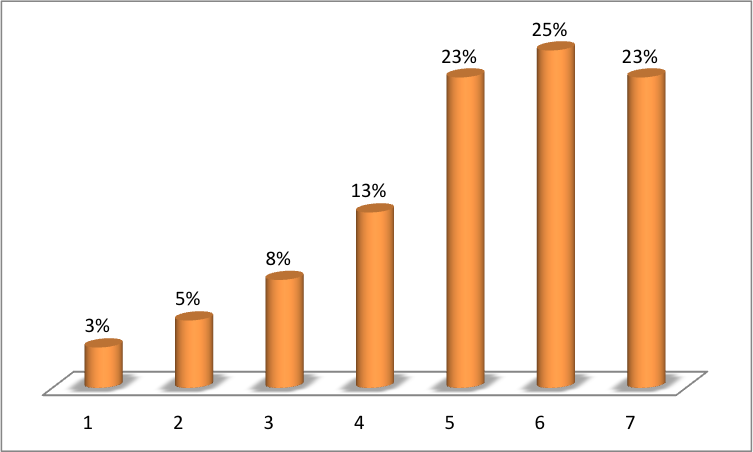
\includegraphics[width=0.9\columnwidth]{survey-q-4.png}
\caption{Distribution of 247 responses to ``did you find confer personalized schedule helpful? Did it make navigation easier?''}
\label{survey-q-4}
\end{subfigure}

\vspace{10pt}
\begin{subfigure}[t]{0.9\columnwidth}
\centering
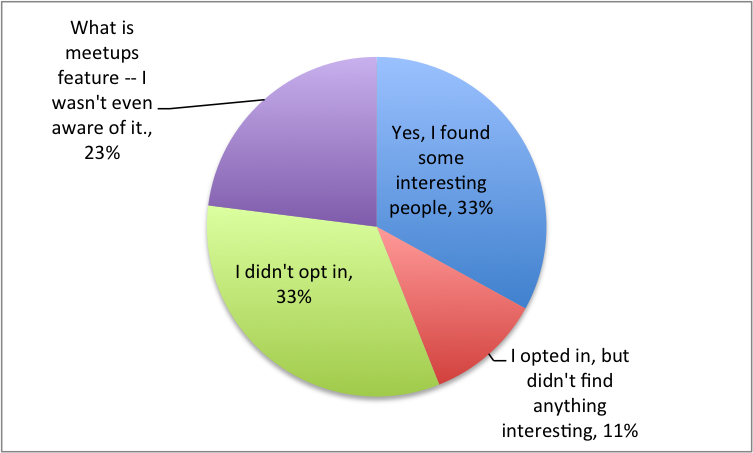
\includegraphics[width=0.9\columnwidth]{survey-q-5.png}
\caption{Distribution of 103 responses to ``what was your experience with the confer meetups feature?''}
\label{survey-q-5}
\end{subfigure}


\caption{Survey Results (all ratings are on 1-7 likert scale)}
\label{survey-responses}
\end{figure}

We look at the survey responses along with the usage statistics in the context of the three design goals we described earlier.

\textbf{Confer helps attendees discover relevant papers/talks.}\\
We asked attendees to rate the relevance and usefulness of Confer recommendations on 1-7 likert scale (Figure~\ref{survey-q-2}). 74\% of the respondents rated it as 5 or above. Only 19\% of the respondents gave a 3 or below rating. We also asked the attendees if the recommendations helped them discover new interesting papers.  A large majority (83\% of the respondents) responded with a `Yes'.

Log analysis suggests that on an average 63.8\% (median 66.45, std-dev: 14.76) of the papers an attendee has marked as ``interested in seeing'' come from clicking on recommendations. This shows that a huge fraction of what an attendee could be interested in seeing was covered by Confer recommendations.

Recommendations are tricky to get right. While most respondents found the recommendations relevant and useful, a few respondents mentioned in their comments that they expected the recommendations to show papers outside their interest areas too. Our current recommendation approach generates recommendations for an attendee based on only the interests inferred from all the papers already marked by the attendee. It would be interesting to explore the effect of adding diverse recommendations.

\textbf{Confer helps attendees find and meet other attendees with shared interests.}\\
Meetups was active for only three conferences and thus we consider only those respondents (103) who registered for one of these conferences. 23\% of the respondents responded that they were not aware of it and 33\% didn't opt in. Out of the remaining (44\% of 103 = 45), 33\% did find other attendees with similar interests (Figure~\ref{survey-q-5}). 11\% said they didn't find anything interesting.

Out of the 45 respondents who opted in, 56\% initiated a communication with other attendees recommended to them by Confer. 52\% of the respondents said they got contacted by other attendees.

From the log analysis we find 436 users (21.8\% of the total registered users) who explicitly enabled the Meetups functionality. There are 139 pairs with both-way favoriting (a pair favorited each other), and 179 pairs with one-way favoriting (only one side favorited the other in a pair).

Both the log analysis and the survey results suggest that Meetups wasn't used as much as we'd like. The low Meetups usage could be because of the following reasons: 
\begin{itemize}
\item Because of privacy considerations, we kept everyone ``opted out'' as default which affected the number of users who can appear in the recommendation lists of attendees. Attendees discovered this feature either by word of mouth, or by clicking on the Meetup link.
\item A possible reason for one-way favoriting could be due to the fact that many attendees favorite famous professors/researchers -- these famous professors/researchers often tend not to respond to unsolicited meeting requests.
\end {itemize}

\textbf{Confer helps attendees navigate using a personalized schedule.}\\
We asked if the personalized schedule was helpful and if it helped them in navigating the conference. 71\% of the respondents gave a 5 or above rating on 1-7 likert scale (Figure~\ref{survey-q-4}). Only 16\% of the respondents gave a 3 or below rating. Our log analysis suggests that 83\% of the attendees visited the personalized schedule page at least once during the conference days.

Many respondents mentioned in their comment that they expect more features such as export to calendar, reminders, etc. integrated with the personalized schedule.

\section{A Case For A Data-Driven Decision Making}
Now we shift our focus to analyzing how the data gathered from the usage of Confer can be used to help conference organizing committee in various activities such as scheduling sessions, choosing speakers, creating program committees, planning community interactions, etc. In this paper, we argue for a data-driven approach towards conference planning. We did an experiment for CHI 2014 to understand if it is feasible to gather enough data before the conference that can be helpful to the organizing committee. 
\subsection{CHI 2014 Experiment}
For CHI 2014, the program chairs released the list of accepted papers (Figure~\ref{all-accepted-papers}) on Confer 4 months before the conference (45 days before releasing the sessions and schedule). It was simply a list of papers with no sessions and schedule information. The CHI 2014 organizing committee also ensured that the first list of papers was \emph{only} available on Confer. The chairs made an official announcement on Twitter (Figure~\ref{chi-announcement-2}) that attendees can explore and mark the papers they want to see at the conference. They also announced that the preferences collected from Confer would be used for optimal session planning (Figure~\ref{chi-announcement-1}). Conference attendees marked papers they want to see at the conference (Figure~\ref{attendee-response}) by either searching (Figure~\ref{confer-search}) or using recommendations (Figure~\ref{confer-recommendations}).

\begin{figure}[!h]
\centering
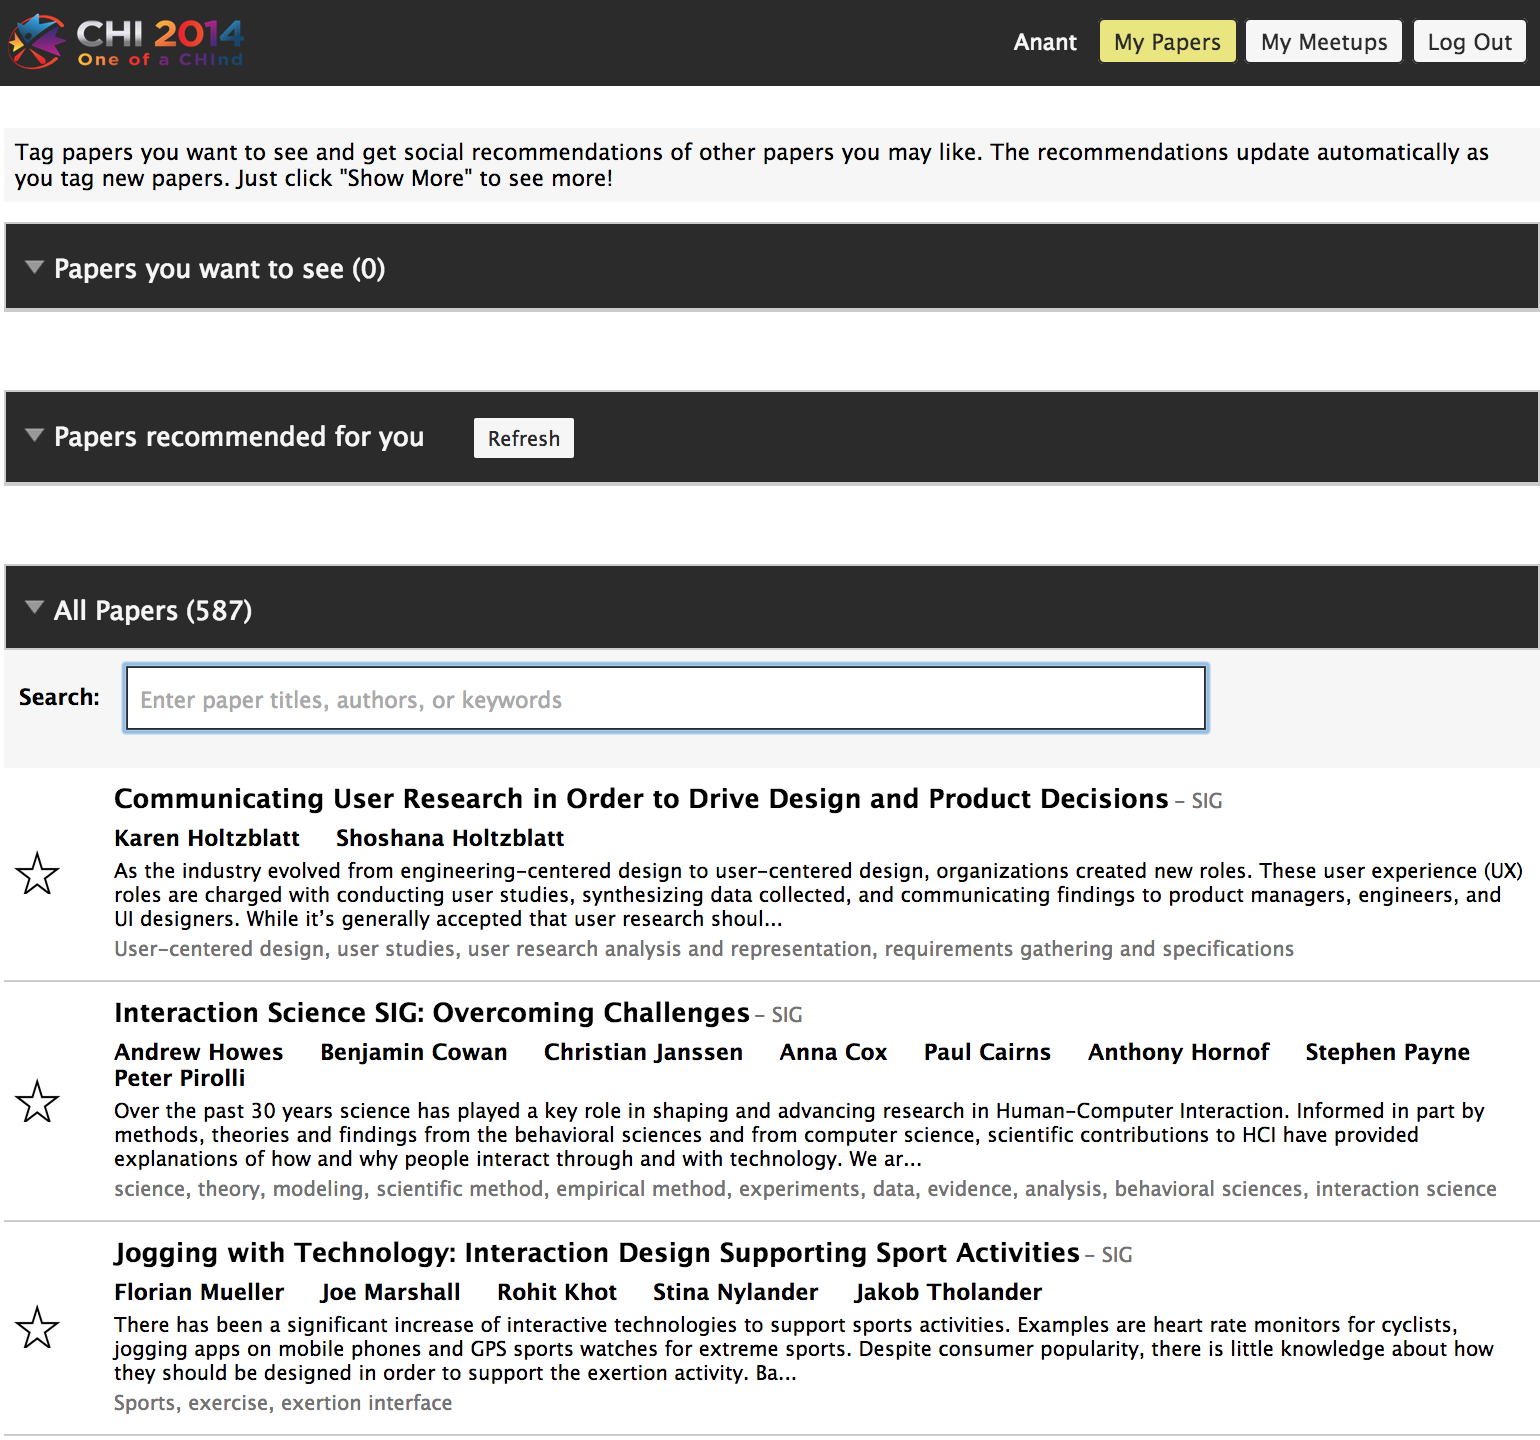
\includegraphics[width=0.95\columnwidth]{all-accepted-papers.png}
\caption{For CHI 2014, all the accepted papers were released on Confer 4 months before the conference (45 days before releasing the schedule).}
\label{all-accepted-papers}
\end{figure}

\begin{figure}[!h]
\centering
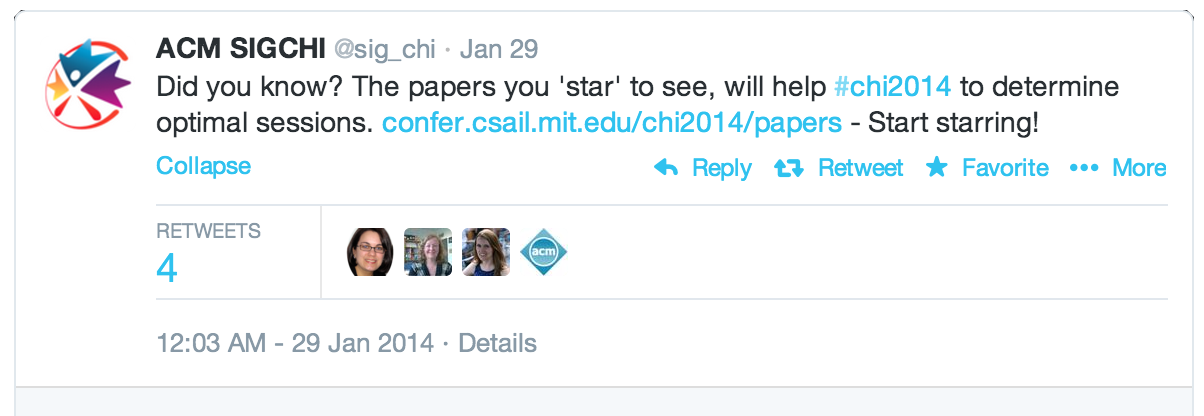
\includegraphics[width=0.95\columnwidth]{chi-announcement-1.png}
\caption{CHI announcement on Twitter: ``attendees' preference would be used to create optimal sessions''}
\label{chi-announcement-1}
\end{figure}

The primary motivation for attendees was to get an early preview of all the accepted papers which they can explore and interact with. From our logs we find that attendees search for papers from a particular institution/organization, papers by a particular author, papers related to a particular topic, etc. They spend time exploring different papers by clicking the recommendations we show. While exploring, they add interesting papers to their preference list. The Confer interface and underlying recommendation engine are designed to support the exploratory behavior and keep the attendees engaged by showing them papers they are most likely to find interesting. To encourage participation, after releasing the accepted papers on Confer, CHI officially announced that attendees should explore CHI 2014 papers on Confer (Figure~\ref{chi-announcement-2}). CHI also put Confer links in all the official announcements for honorable mention and best paper awards. 

\begin{figure}[!h]
\centering

\includegraphics[width=0.95\columnwidth]{chi-announcement-2.png}
\caption{CHI announcement on Twitter: ``Attendees can explore CHI 2014 papers on Confer''}
\label{chi-announcement-2}
\end{figure}

Another inherent motivation for attendees was that they want a schedule which takes into account their preferences (Figure~\ref{chi-announcement-1}) so that they can see all the papers they want to see without any conflict. A conflict is when two papers that an attendee wants to see are scheduled at the same time. To motivate attendees, CHI officially made an announcement that the data collected from Confer would be used to determine the optimal sessions.



\begin{figure}[!h]
\centering
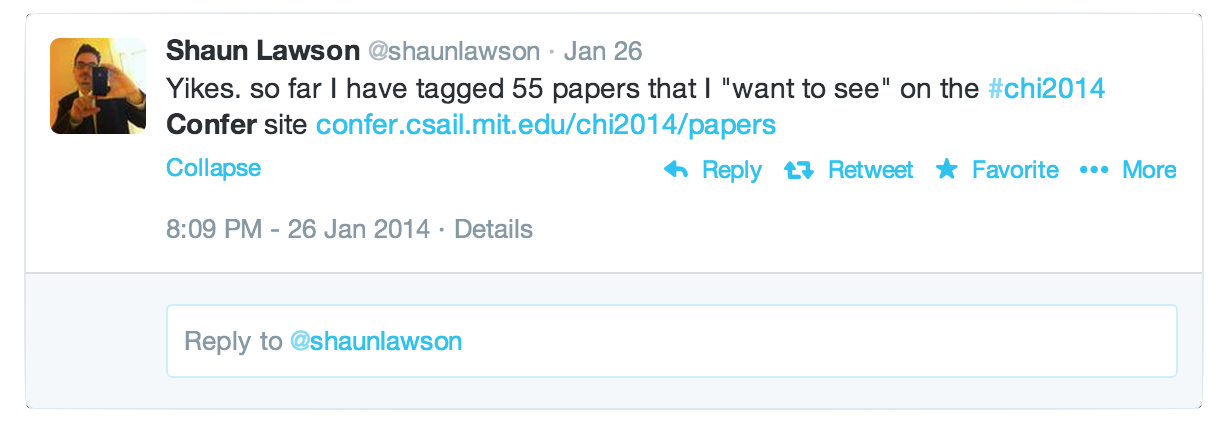
\includegraphics[width=0.95\columnwidth]{attendees-response.png}
\caption{An attendee tweets about his ``wants to see'' list for CHI 2014}
\label{attendee-response}
\end{figure}

We saw a really good response from attendees (Figure~\ref{attendee-response}). For CHI 2014, during those 45 days, 347 attendees marked 7228 preferences in total \emph{(mean: 20.83, median: 14, std-dev: 21.47, min: 1, max: 156)}. It covered 581 papers (98.98\% of all the accepted papers). On an average, each paper was in the preference list of 12.44 attendees \emph{(mean: 12.44, median: 10, std-dev: 7.98, min: 1, max: 56)}. While this number might look too small (12\% of the total attendance), we find that after a certain threshold, the similarity structure doesn't change much even if we get data from more attendees. We however agree that more the early participation is, more confident the conference organizing committee would be in making decisions based on the data.

The data collected from Confer was used by CHI organizing committee for making various decisions for CHI 2014. Along with Cobi's author-sourcing data, the data collected from Confer was fed into Cobi's scheduling tool to optimally plan sessions. The data was also used to get a sense of popular papers in advance.

\subsection {Data-Driven Decision Making Use-Cases}
We saw an active participation for CHI 2014. We believe that with organizational support, enough data can be gathered prior to holding (or scheduling) a conference. Now we present various use-cases for which the data collected from Confer usage could be useful. 

\emph{Create Coherent Sessions.} If many attendees want to see a pair of papers together, then the two papers can be categorized as related. Ideally, it would make sense to put a set of papers a lot of attendees want to see together in the same session. Sessions can be generated by creating clusters based on shared-interests.

\emph{Reduce Conflicts.} This is straight-forward -- don't schedule two papers in different sessions at the same time if many attendees want to see both of them.

\emph{Measure Paper Popularity.} Determining paper popularity in advance is useful for making various decisions on the organizers' side. For example, when assigning rooms, organizers can put popular papers in bigger rooms, and less popular papers in smaller rooms. More accurate popularity estimates can avoid situations like Figure~\ref{crowded-room}, which shows a session from CHI 2013 when a paper a lot of attendees wanted to see was assigned a smaller room. An alternative strategy for scheduling would be as follows: assign a paper very few people want to see in a session with more popular papers, rather than clustering all the less popular papers in the same session. This can help conference organizers maintain popularity balance in the schedule.

\begin{figure}[!h]
\centering
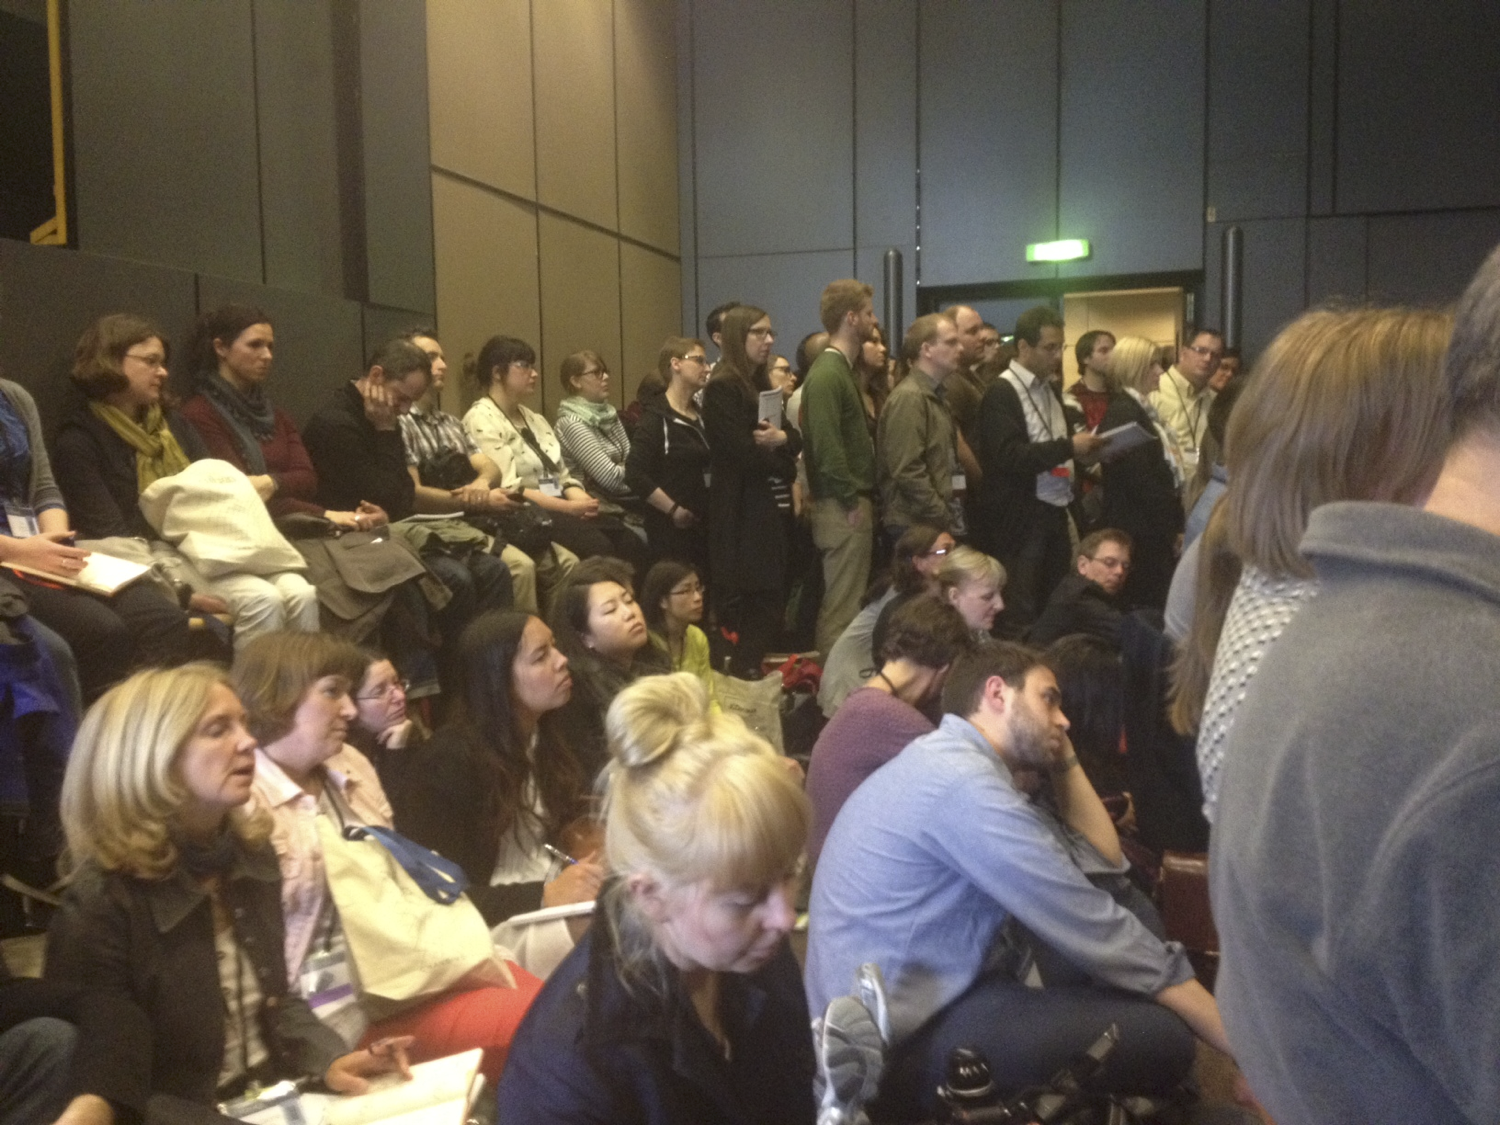
\includegraphics[width=0.95\columnwidth]{crowded-room.png}
\caption{CHI 2013: A popular paper scheduled in a small room}
\label{crowded-room}
\end{figure}

\emph{Understanding Community:} The data collected from Confer is useful not just for creating sessions and schedule but for making strategic decisions. The data can be used to understand the community structure -- specifically the areas of interest and the connections between them. It provides rich preference data that can be used to detect networks within the community and understand the connections within and outside the network.

Figure~\ref{chi2013-community-view-10} shows the major communities detected using Confer data for CHI 2013. We see education, crowdsourcing, and social media communities very much connected but have very little connection with hardware communities. It does not make sense to run education, crowdsourcing, and social media sessions in parallel. We also see hardware communities very strongly connected within themselves but don't have many connections outside the community.  On the other hand, the design research community connects to every other community. These insights can help conference organizers make important decisions for planning future conferences and community interactions.
\begin{figure}[!h]
\centering
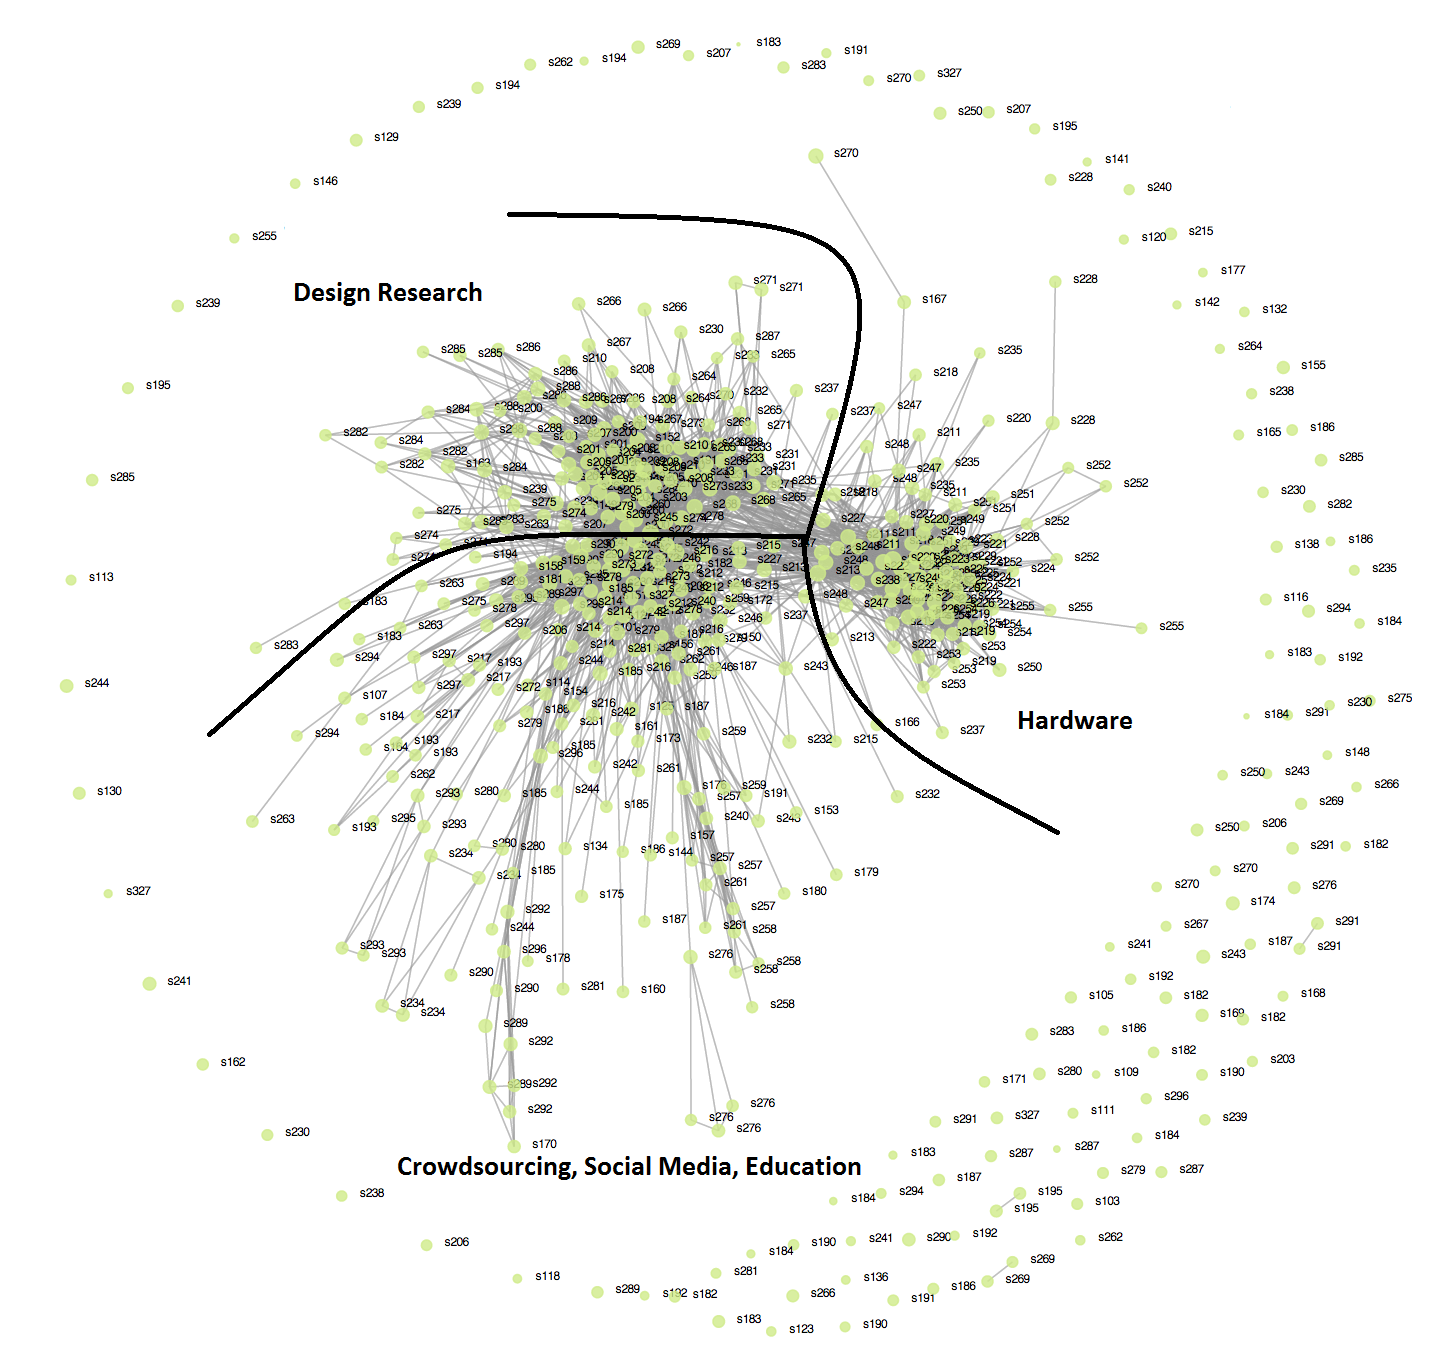
\includegraphics[width=0.95\columnwidth]{chi2013-community-view-10.png}
\caption{CHI 2013 Community Structure: 3 major communities emerge from CHI 2013 by clustering confer preference data.}
\label{chi2013-community-view-10}
\end{figure}

A good understanding of the community network can also be useful in discovering new areas of research and practice, new methodologies, and emerging application areas. After zooming in, we find that within the hardware community there are smaller sub-communities such as gesture, multitouch etc. We observe many emerging communities such as pointing devices, accessibility, analytics, etc.  Many of these smaller sub-communities are officially not recognized as a sub-community within CHI. We believe that conference organizing committee would benefit from the insights that we can gain by mining the usage data.

\begin{figure}[!h]
\centering
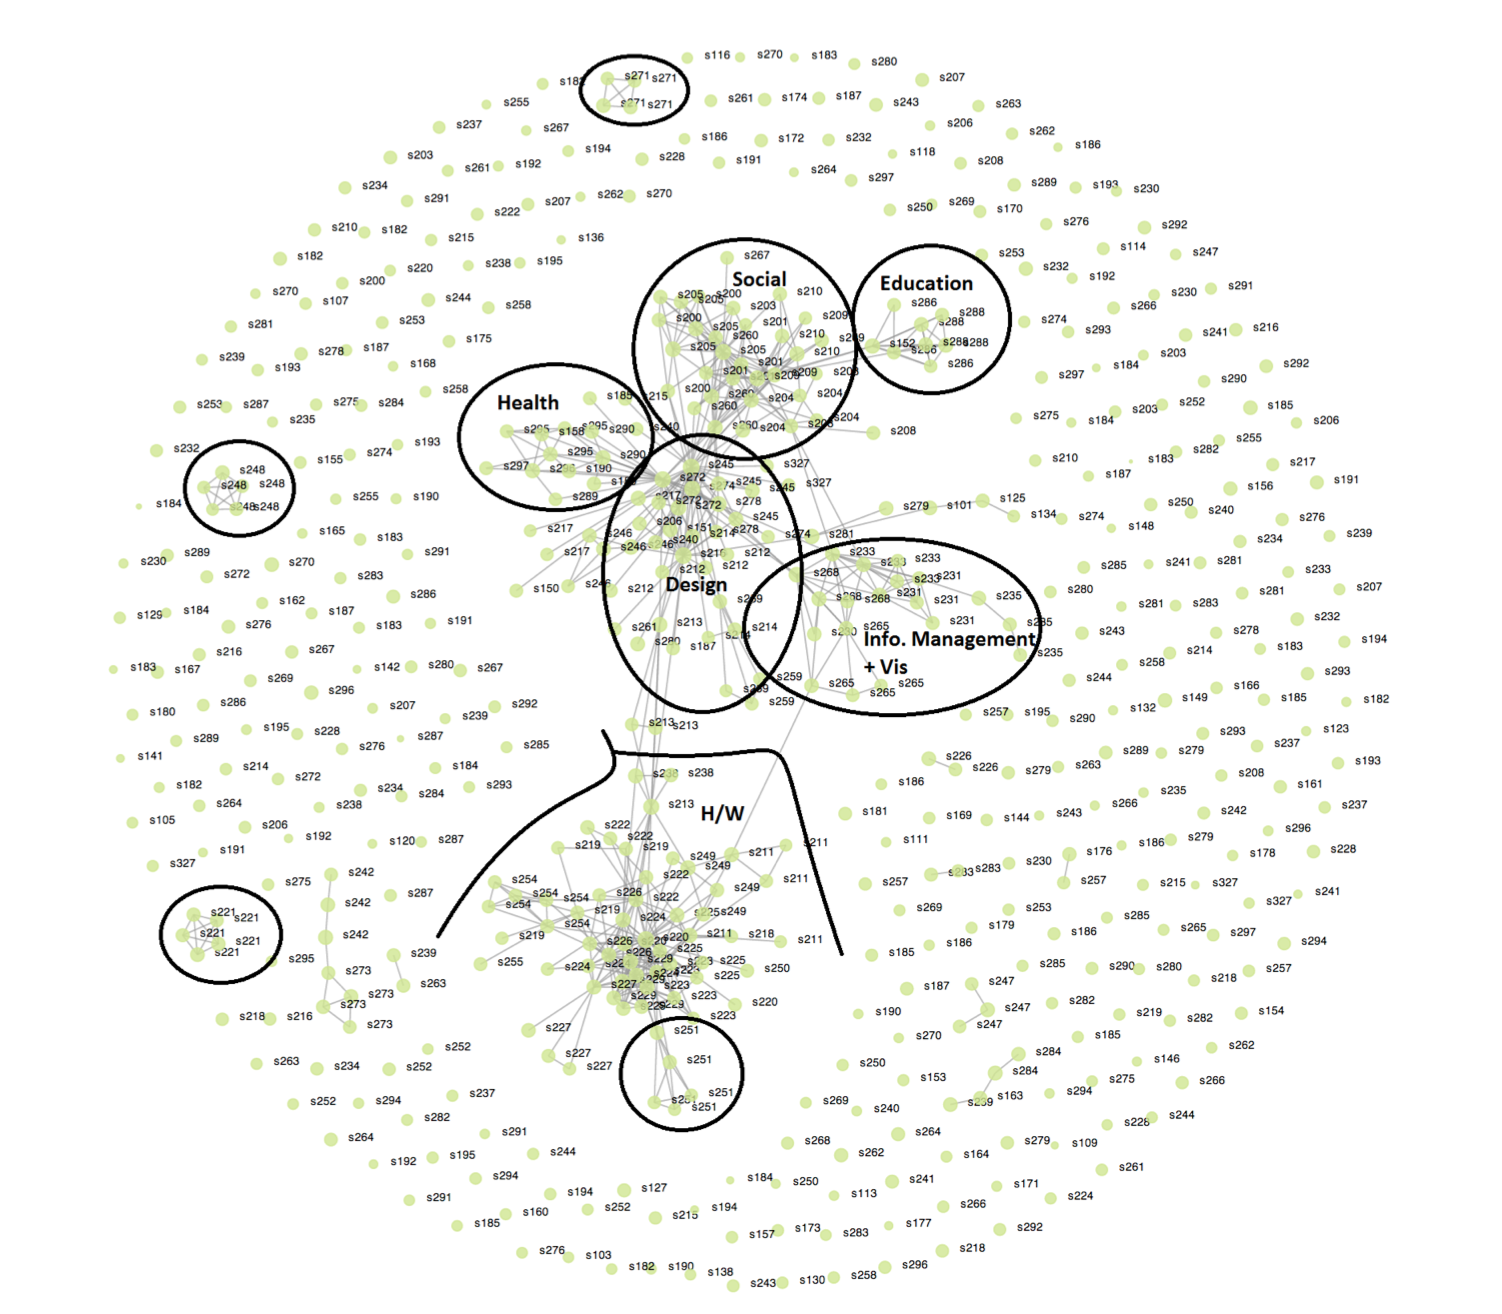
\includegraphics[width=0.95\columnwidth]{chi2013-community-view-15.png}
\caption{CHI 2013 Community Structure: smaller sub-communities emerge by refining the clusters}
\label{chi2013-community-view-15}
\end{figure}

\section{Discussion}
One interesting aspect of this paper is to look at how data collected as a by-product of a natural exploration by conference attendees can be useful for making various decisions in conference planning. Attendees use the tool for their own benefit, but the collective data can help organizers and the community. Our CHI 2014 experiment was a proof of concept demonstrating that it is possible to gather a rich preference data well in advance that it can be used for creating sessions and schedule, choosing speakers, planning rooms, etc. The preference data is valuable for scheduling, ensuring that sessions drew together individuals with shared interests, and that conflicts between papers with the same audience were minimized.  Detecting communities of interest could be useful for deciding panels. Specific to CHI community, birds-of-a-feather gatherings could be organized to discuss the papers and topics of greatest interest within each sub-community.

Confer data has also been used by other tools/applications targeting conference attendees. 
CommonTies ~\cite{Abouzied:2014:CCN:2556420.2556783}, a simple technological nudge that uses context-aware profile-matching system to encourage social interactions among strangers was deployed at CSCW 2014. The profile matching system of CommonTies was powered by Confer Meetups APIs. Confer APIs allow researchers and practitioners to build new applications that can make use of the Confer data.

While the data from only a fraction of attendees cannot give a complete picture of interests at the conference, we find that after a certain threshold, the similarity structure doesn't change much even if we get data from more attendees. We however agree that more the early participation is, more confident the conference organizing committee would be in making decisions based on the data. We saw that if conference organizers explicitly pursue gathering this data prior to holding (or scheduling) the conference, then a far higher rate of data gathering can be achieved.

It's worth mentioning the flip side too though -- the preferences marked by attendees could be susceptible to external influence such as Confer recommendations, social trends (links shared on social media by friends), CHI award/honorable mention tweets, etc. While the current system doesn't take any special care for external influences, we can model some of these influences by looking at the referer page and other HTTP parameters.

\section{Conclusion}
Confer is a tool that collects natural, rich preference data on how attendees plan to spend their time at the conference. While the tool is useful for conference attendees to discover relevant papers/talks, navigate using a personalized schedule, and meet other attendees with shared interests, the data collected from the usage of the tool can be mined to gain deeper insights into the structure of shared interests, community, sub-communities, different areas of research, new/emerging areas, etc. Our experiment at CHI 2014 demonstrates that with some help from conference organizers, it is possible to collect attendees' preference data prior to holding (or scheduling) the conference so that it is useful for creating sessions and schedule, room planning, etc. We show how data-driven technique can help conference organizers gain deeper insights into the structure of shared interests, community, sub-communities, different areas of research, new/emerging areas, etc. which can be useful for future conferences and community interactions.


% Balancing columns in a ref list is a bit of a pain because you
% either use a hack like flushend or balance, or manually insert
% a column break.  http://www.tex.ac.uk/cgi-bin/texfaq2html?label=balance
% multicols doesn't work because we're already in two-column mode,
% and flushend isn't awesome, so I choose balance.  See this
% for more info: http://cs.brown.edu/system/software/latex/doc/balance.pdf
%
% Note that in a perfect world balance wants to be in the first
% column of the last page.
%
% If balance doesn't work for you, you can remove that and
% hard-code a column break into the bbl file right before you
% submit:
%
% http://stackoverflow.com/questions/2149854/how-to-manually-equalize-columns-
% in-an-ieee-paper-if-using-bibtex
%
% Or, just remove \balance and give up on balancing the last page.
%
\balance

\bibliographystyle{acm-sigchi}
\bibliography{references}
\end{document}
